% Created 2021-03-22 Mon 16:21
% Intended LaTeX compiler: pdflatex
\documentclass[a4paper,11pt]{article} [NO-DEFAULT-PACKAGES] \usepackage{wx672hyperref}
\usepackage{amsmath,amsfonts,amssymb}
\usepackage{graphicx}
% \usepackage[table]{xcolor}
\usepackage[margin=0.9in,bmargin=1.0in,tmargin=1.0in]{geometry}
% \usepackage{algorithm2e}
\usepackage{listings}
\usepackage{algorithm}
\usepackage{amsmath}
\usepackage{arydshln}
\usepackage{subcaption}
\usepackage[backend=bibtex,sorting=none]{biblatex}
\newcommand{\point}[1]{\noindent \textbf{#1}}
\usepackage{hyperref}
\usepackage{csquotes}
\usepackage{graphicx}
% \usepackage{subfig}
\usepackage[mla]{ellipsis}
\parindent = 0em
\setlength\parskip{.5\baselineskip}
\usepackage{xeCJK}
\author{葛宇航 2020111071}
\date{2021-03-22}
\title{《最优化方法》 实验报告 01}
\hypersetup{
 pdfauthor={葛宇航 2020111071},
 pdftitle={实验报告},
 pdfkeywords={latex, org-mode, writing},
 pdfsubject={my org-mode to latex templates},
 pdfcreator={Emacs 26.1 (Org mode 9.1.9)}, 
 pdflang={English}}
\begin{document}

\lstset{
 columns=fixed,       
 numbers=left,                                        % 在左侧显示行号
 numberstyle=\tiny\color{gray},                       % 设定行号格式
 frame=none,                                          % 不显示背景边框
 backgroundcolor=\color[RGB]{245,245,244},            % 设定背景颜色
 keywordstyle=\color[RGB]{40,40,255},                 % 设定关键字颜色
 numberstyle=\footnotesize\color{darkgray},           
 commentstyle=\it\color[RGB]{0,96,96},                % 设置代码注释的格式
 stringstyle=\rmfamily\slshape\color[RGB]{128,0,0},   % 设置字符串格式
 showstringspaces=false,                              % 不显示字符串中的空格
 language=python,                                        % 设置语言
}

\maketitle
编程语言: Python

开发环境: Linux - Pycharm 2020


\section*{斐波那契搜索}
\label{sec:org9b4ea6a}
计算函数 \(y = x**2 + x - 2\) 在区间[-1, 3]上的极值:

对应代码: fibo\_solve.py

运行结果:
\begin{center}
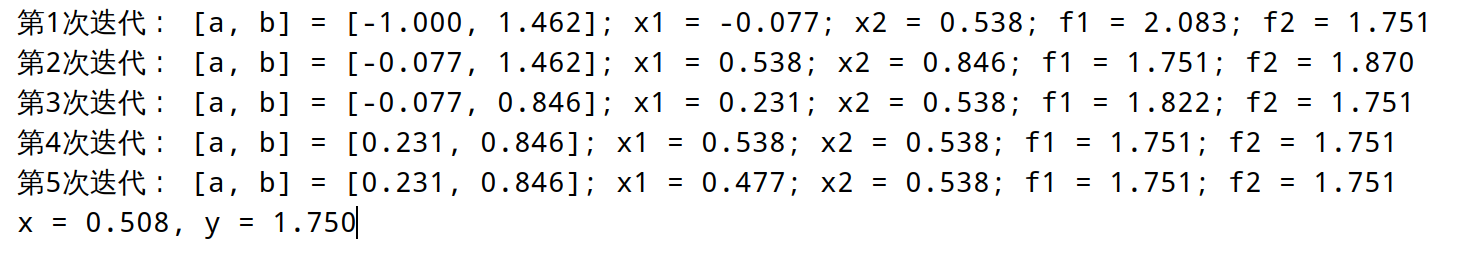
\includegraphics[width=0.8\linewidth]{2021-03-22_15-57-11_screenshot.png}
\end{center}

\section*{黄金分割点搜索}
\label{sec:orgaf2f859}
计算函数 \(y = x**2 + x - 2\) 在区间[-1, 3]上的极值:

对应代码: gold\_solve.py

运行结果:
\begin{center}
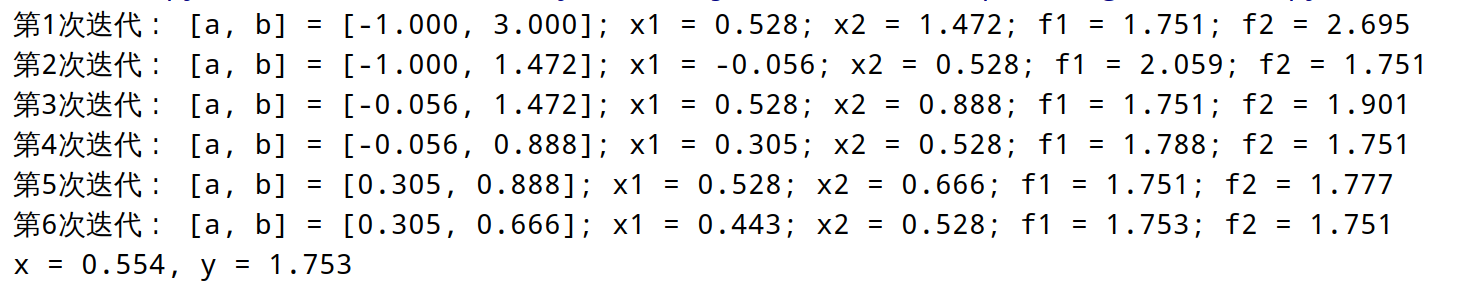
\includegraphics[width=0.8\linewidth]{2021-03-22_15-56-41_screenshot.png}
\end{center}


\section*{进退法}
\label{sec:org3876c12}
计算函数 \(y = x**2 + x - 2\) 的可能区间, 并在求的的区间上求解极值:

对应代码: advance\_retreat.py

运行结果:
\begin{center}
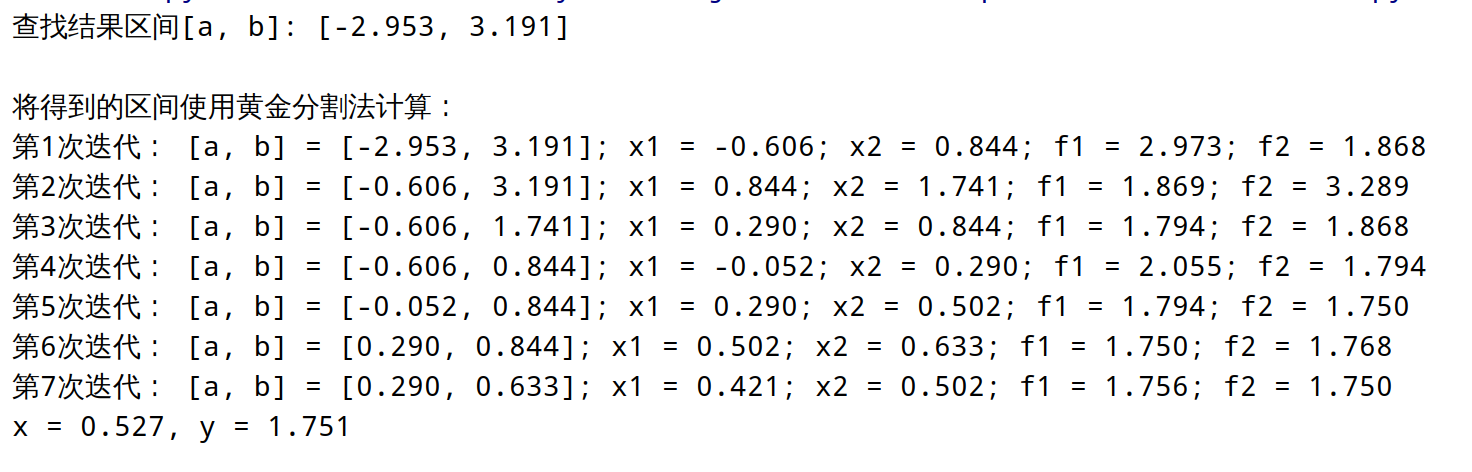
\includegraphics[width=0.8\linewidth]{2021-03-22_16-04-15_screenshot.png}
\end{center}
\end{document}
